% costante_eulero_mascheroni.tex
%! TeX root = ../lezione_turbo.tex
\chapter{Costante di Eulero-Mascheroni}
Durante il corso è stato dimostrato che la serie armonica $s_n= \sum^n_1 \frac{1}{k}$ è asintotica a $ \log(n)$.

In questa sezione si ricaverà che la loro differenza converge.

\begin{Res} 
	Esiste un reale $ \gamma \in \left( \frac{1}{2},1 \right)$ tale che
	\begin{equation*}
		\lim \limits_{n \to+ \infty}s_n- \log(n)= 
		\gamma.
	\end{equation*}
\end{Res}
\begin{proof}
	Il nostro piano è $s_n - \log(n)$ come un integrale, applicare la gamma di strumenti noti, e poi prendere il limite.

	Partiamo da $s_n$. 
	Vogliamo trovare una funzione $F_n$ derivabile e parametrizzata su $n$ tale che $F_n(1)=s_n$ e $F_n(0)=0$. 
	Poi, vogliamo sfruttare questa proprietà per applicare il TFC\footnote{Teorema Fondamentale del Calcolo}, per tradurre la differenza $F_n(1)-F_n(0)$ in un integrale calcolato su un intervallo fisso.
	Consideriamo il polinomio (calato dall'alto\dots)
	\begin{equation*}
		F_n : x \in [0,1] \to
		\sum^n_1 \frac{x^k}{k} \in \mathbb{R},
	\end{equation*}
	che è derivabile e rispetta i vintoli.
	L'integranda sarà la derivata di $F_n$, data da
	\begin{equation}
		\label{res1}
		f_n(x)= 
		\sum^{n-1}_0x^k= 
		\frac{x^n-1}{x-1}.
	\end{equation}	
	Osservando allora che $f$ è continua (quindi integrabile), ricaviamo
	\begin{equation*}
		s_n=
		F(1)-F(0)= 
		\int^1_0f(x) \: \mathrm{d}x= 
		\int^1_0 \frac{1-x^n}{1-x} \: \mathrm{d}x= 
		\int^1_0 \frac{1-(1-y)^n}{y} \: \mathrm{d}x,
	\end{equation*}	
	dove abbiamo applicato il TFC sulla primitiva (per costruzione) $F_n$ di $f_n$, e sostituito $y=1-x$. 
	
	Ora stiamo lavorando nel continuo. Per semplicare l'espressione (idealmente, facendo apparire un $\log n$), applichiamo l'idea della Proposizione \ref{eq_fun_gamma}: spezziamo l'integrale in due, e mostriamo che uno dei due contributi decade.
	In particolare, definiamo
	\begin{gather*}
		s_n = 
		\mathcal{I}_n + \mathcal{J}_n \quad \text{dove} \\
		\mathcal{I}_n = \int^1_0 \frac{1-e^{-nx}}{x} \: \mathrm{d} x 
		\qquad 
		\mathcal{J}_n= \int^1_0 \frac{e^{-nx}-(1-x)^n}{x} \: \mathrm{d} x.
	\end{gather*}
	
	\begin{figure}
		\centering
		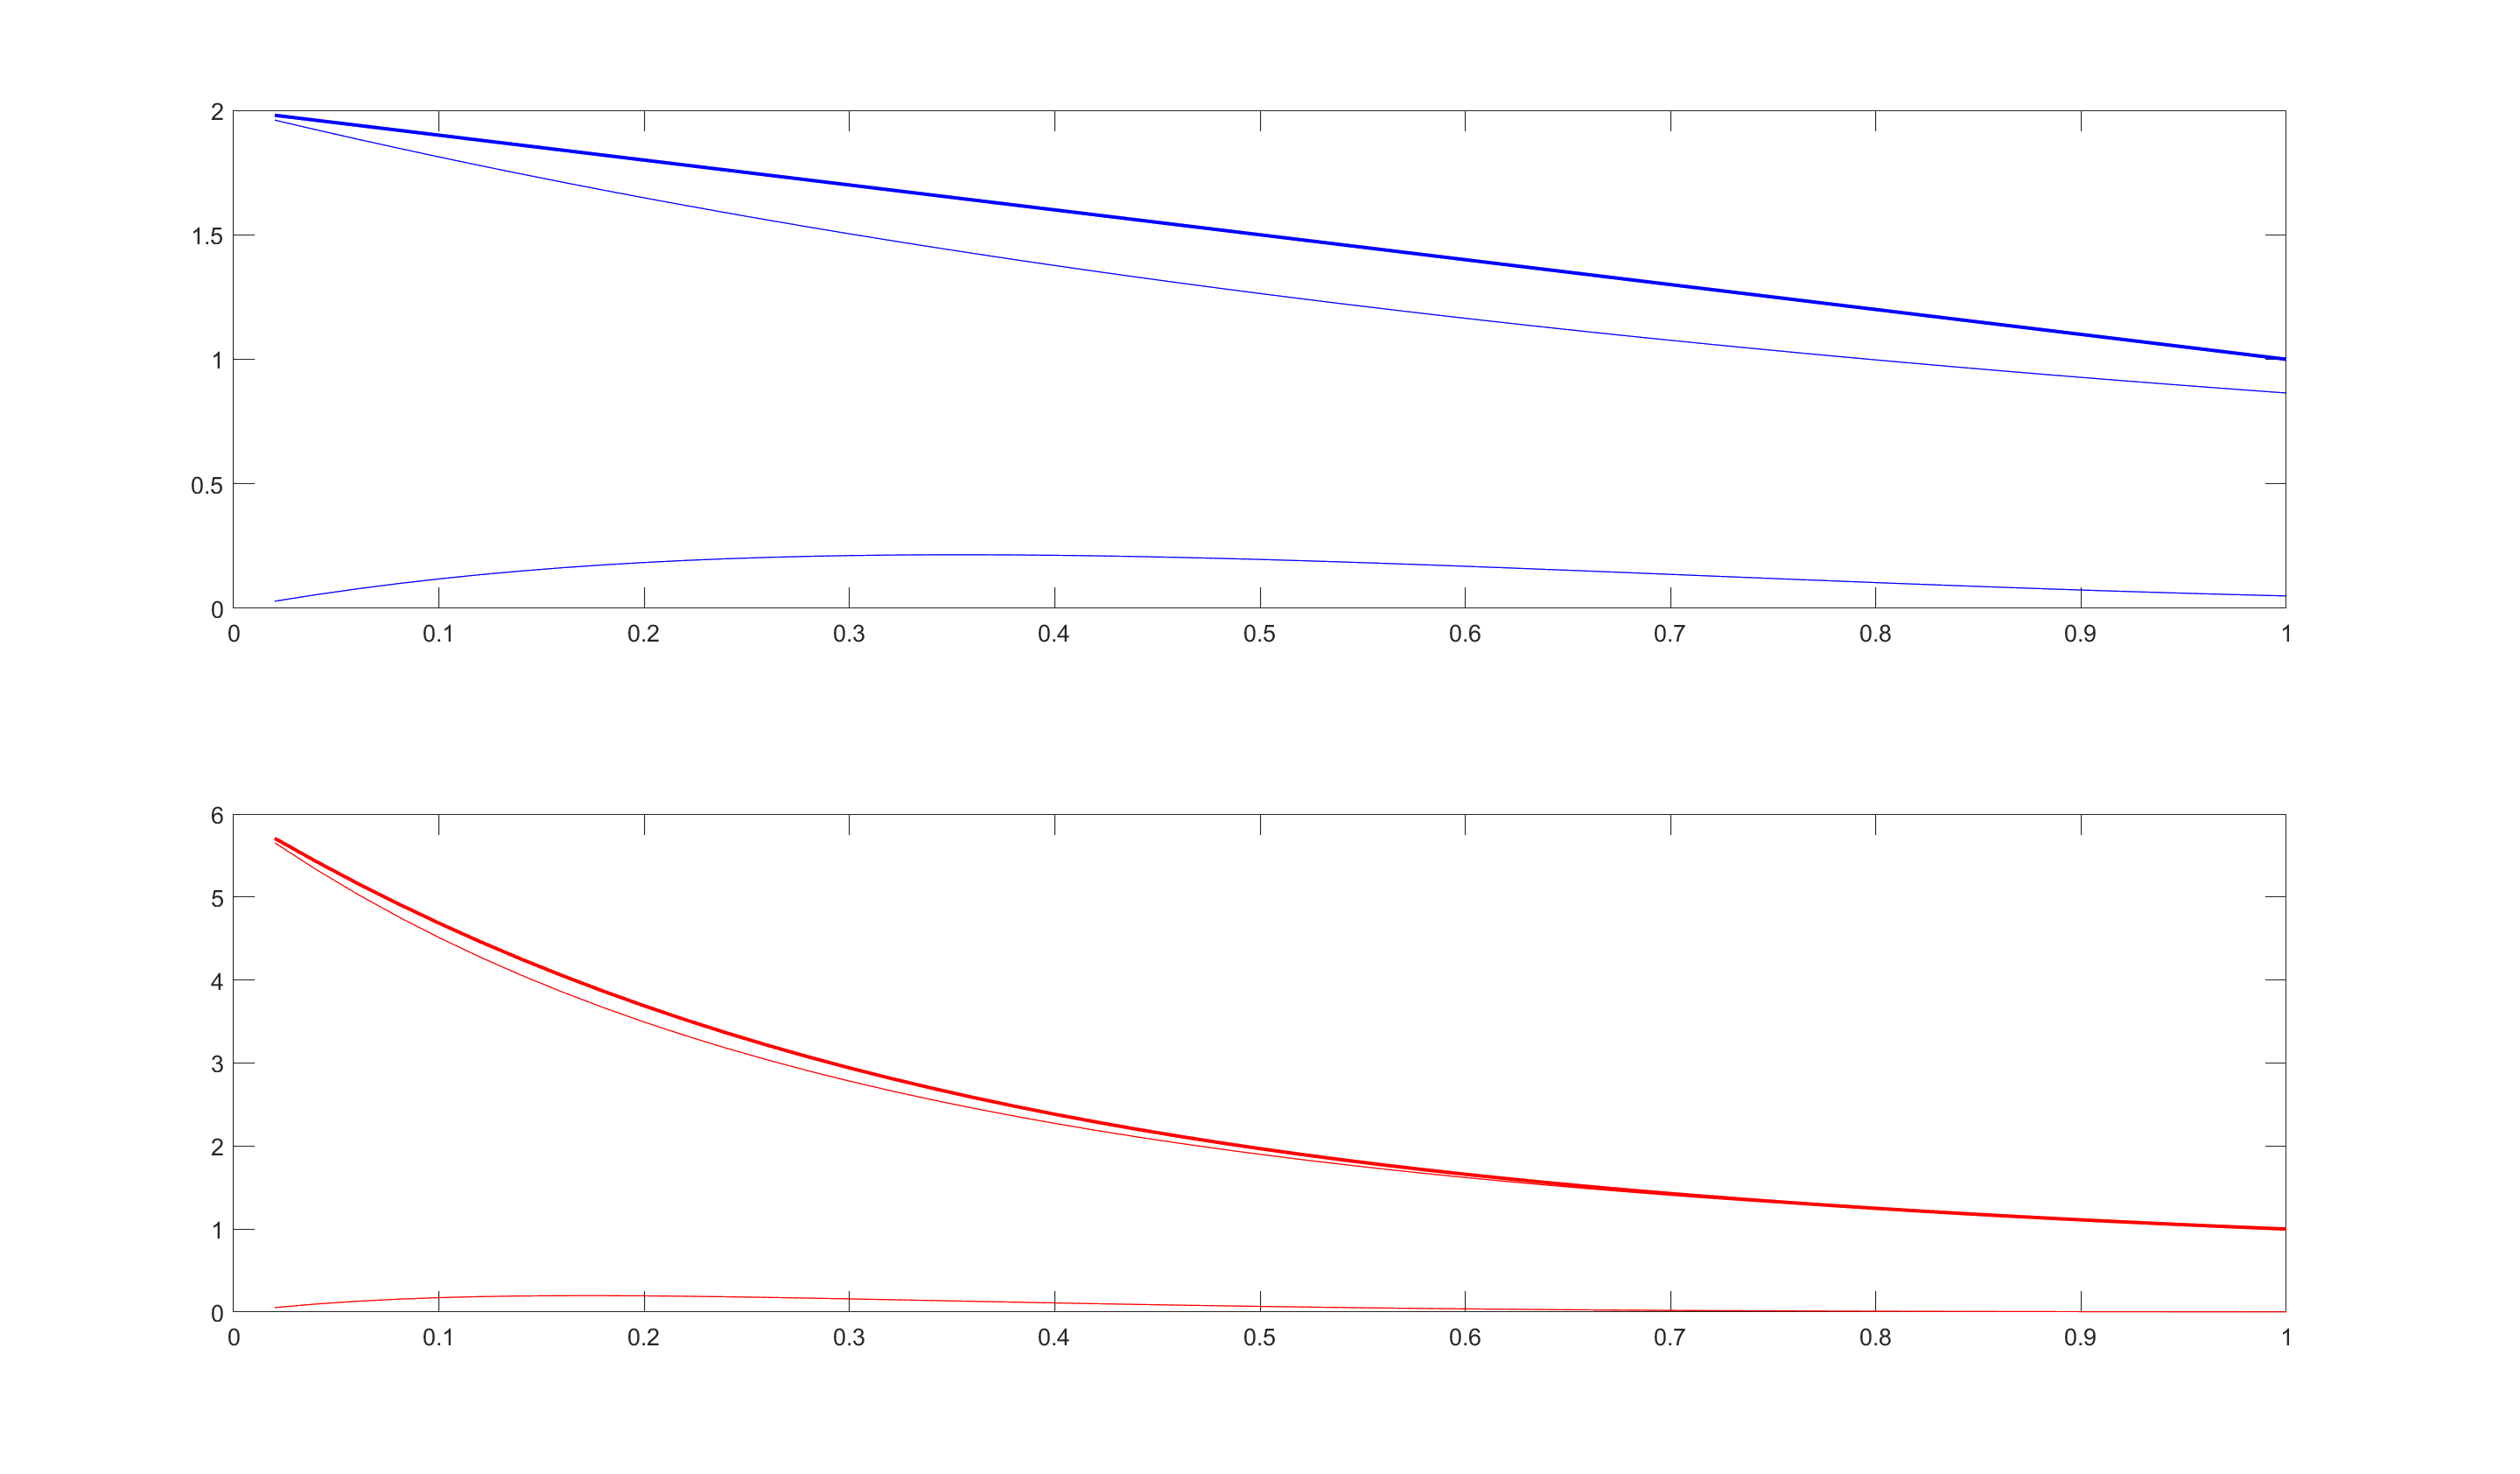
\includegraphics[width=.9\textwidth]{assets/eulero_mascheroni_choice.png}
		\caption{Le tre funzioni integrande ($f_n$ in grassetto), per $n=3$ e per $n=6$}.		
	\end{figure}

	Dalla figura, è chiaro che $\mathcal{J}_n$ decada. 
	A riprova di ciò, se uno considera il limite $f_n(x)$ per ogni $x \in \left( 0,1 \right]$, calcolato espandendo il polinomio di Taylor, trova che si annulla. Per $x=0$ la funzione non è definita, ma può essere estesa con continuità per ogni $n$, secondo il limite
	\begin{equation*}
		\lim \limits_{x \to0} \frac{e^{-nx}-(1-x)^n}{x}= 
		\lim \limits_{x \to0} \frac{o(x)}{x}=
		0,
	\end{equation*}
	calcolato di nuovo sviluppando l'esponenziale con Taylor.

	Questa è un'applicazione immediata del teorema di Convergenza Dominata, ma nello spirito di questa lezione è stato deciso di fare una dimostazione solo di AM1.

	
	
	% Allora, per dei risultati sulle successioni funzionali (in particolare, la convergenza uniforme $f_n \rightrightarrows f$ e continuità di $f_n$), si ottiene che
	% \begin{equation*}
	% 	\lim \limits_{n \to+ \infty} \int^1_0f_n(x) \: \mathrm{d}x= 
	% 	\int^1_0 \lim \limits_{n \to+ \infty}f_n(x) \: \mathrm{d}x=
	% 	\int^1_00 \: \mathrm{d}x=
	% 	0.
	% \end{equation*}

	% In conclusione $ \lim \limits_{n \to+ \infty} \mathcal{J}_n=0$ e si può dimostrare che $ \mathcal{J}_n \sim \frac{1}{2n}$.

	Ora analizziamo $ \mathcal{I}_n$. 
	L'integrale è improprio, e presenterebbe un punto critico in $x=0$. 
	In realtà, l'integranda converge per le gerarchie d'infinito e quindi è integrabile secondo Riemann su tutto l'intervallo.

	L'integrale può essere semplificato fino a raggiungere la forma "$ \log x +f(x)$": si sostituisca $t=nx$ e poi si integri per parti.
	\begin{align*}
			\mathcal{I}_n= 
			\int^1_0 \frac{1-e^{-nx}}{x} \: \mathrm{d}x
			&= 
			\int^n_0 \frac{1-e^{-t}}{t} \: \mathrm{d}t= 
			\\ &= 
			\left[ \left(1-e^{-t} \right) \log t \right]^n_0 - \int^n_0 e^{-t} \log t \: \mathrm{d}t=
			\\ &=
			\log n-e^{-n} \log n- \int^n_0e^{-t} \log t \: \mathrm{d}t.
	\end{align*}

	Sostituendo la precedente identità nella differenza tra $s_n$ e $ \log n$ otteniamo
	\begin{equation*}
		s_n- \log n= 
		\mathcal{J}_n+ \mathcal{I}_n- \log n= 
		\mathcal{J}_n-e^{-n} \log n- \int^n_0 e^{-t} \log t \: \mathrm{d}t.
	\end{equation*}

	Poichè $ \lim_{n \to \infty} \mathcal{J}_n=0$ e $ \lim_{n \to \infty} e^{-n} \log n=0$, si ricava una formula che permette di trovare la costante con precisione arbitraria:
	\begin{equation*}
		\gamma= 
		\lim \limits_{n \to+ \infty}(s_n- \log n)=
		- \int^{+ \infty}_0e^{-t} \log t \: \mathrm{d}t.
	\end{equation*}

	Un'osservazione interessante, infine, è che questo integrale può essere ricondotto alla Funzione Gamma.	
	Infatti, la derivata $ \Gamma'(x)$, calcolata applicando il Teorema di Lebesegue (e cioè invertendo l'ordine di derivazione e integrazione), soddisfa la relazione
	\begin{align*}
		\Gamma'(x)&= 
		\frac{ \mathrm{d}}{ \mathrm{d}x} \left( \int^{+ \infty}_0e^{-t} \: t^{ \,x-1} \mathrm{d}t \right) = 
		\\ &= 
		\int^{+ \infty}_0 \frac{ \mathrm{d}}{ \mathrm{d}x} \left( e^{-t} \: t^{ \,x-1} \right) \mathrm{d}t= 
		\\ &= 
		\int^{+ \infty}_0e^{-t} \: t^{ \,x-1} \log t \: \mathrm{d}t
	\end{align*}
	Da cui si deduce che $ \gamma=- \Gamma'(1)$, che numericamente equivale a $0,577 \dots$
\end{proof}
\pagebreak